\documentclass[12pt,]{article}
\usepackage{lmodern}
\usepackage{amssymb,amsmath}
\usepackage{ifxetex,ifluatex}
\usepackage{fixltx2e} % provides \textsubscript
\ifnum 0\ifxetex 1\fi\ifluatex 1\fi=0 % if pdftex
  \usepackage[T1]{fontenc}
  \usepackage[utf8]{inputenc}
\else % if luatex or xelatex
  \ifxetex
    \usepackage{mathspec}
  \else
    \usepackage{fontspec}
  \fi
  \defaultfontfeatures{Ligatures=TeX,Scale=MatchLowercase}
    \setmainfont[]{Times New Roman}
\fi
% use upquote if available, for straight quotes in verbatim environments
\IfFileExists{upquote.sty}{\usepackage{upquote}}{}
% use microtype if available
\IfFileExists{microtype.sty}{%
\usepackage{microtype}
\UseMicrotypeSet[protrusion]{basicmath} % disable protrusion for tt fonts
}{}
\usepackage[margin=2.54cm]{geometry}
\usepackage{hyperref}
\hypersetup{unicode=true,
            pdftitle={Chemical Effects on Mammals},
            pdfauthor={Caroline Reents},
            pdfborder={0 0 0},
            breaklinks=true}
\urlstyle{same}  % don't use monospace font for urls
\usepackage{color}
\usepackage{fancyvrb}
\newcommand{\VerbBar}{|}
\newcommand{\VERB}{\Verb[commandchars=\\\{\}]}
\DefineVerbatimEnvironment{Highlighting}{Verbatim}{commandchars=\\\{\}}
% Add ',fontsize=\small' for more characters per line
\usepackage{framed}
\definecolor{shadecolor}{RGB}{248,248,248}
\newenvironment{Shaded}{\begin{snugshade}}{\end{snugshade}}
\newcommand{\KeywordTok}[1]{\textcolor[rgb]{0.13,0.29,0.53}{\textbf{#1}}}
\newcommand{\DataTypeTok}[1]{\textcolor[rgb]{0.13,0.29,0.53}{#1}}
\newcommand{\DecValTok}[1]{\textcolor[rgb]{0.00,0.00,0.81}{#1}}
\newcommand{\BaseNTok}[1]{\textcolor[rgb]{0.00,0.00,0.81}{#1}}
\newcommand{\FloatTok}[1]{\textcolor[rgb]{0.00,0.00,0.81}{#1}}
\newcommand{\ConstantTok}[1]{\textcolor[rgb]{0.00,0.00,0.00}{#1}}
\newcommand{\CharTok}[1]{\textcolor[rgb]{0.31,0.60,0.02}{#1}}
\newcommand{\SpecialCharTok}[1]{\textcolor[rgb]{0.00,0.00,0.00}{#1}}
\newcommand{\StringTok}[1]{\textcolor[rgb]{0.31,0.60,0.02}{#1}}
\newcommand{\VerbatimStringTok}[1]{\textcolor[rgb]{0.31,0.60,0.02}{#1}}
\newcommand{\SpecialStringTok}[1]{\textcolor[rgb]{0.31,0.60,0.02}{#1}}
\newcommand{\ImportTok}[1]{#1}
\newcommand{\CommentTok}[1]{\textcolor[rgb]{0.56,0.35,0.01}{\textit{#1}}}
\newcommand{\DocumentationTok}[1]{\textcolor[rgb]{0.56,0.35,0.01}{\textbf{\textit{#1}}}}
\newcommand{\AnnotationTok}[1]{\textcolor[rgb]{0.56,0.35,0.01}{\textbf{\textit{#1}}}}
\newcommand{\CommentVarTok}[1]{\textcolor[rgb]{0.56,0.35,0.01}{\textbf{\textit{#1}}}}
\newcommand{\OtherTok}[1]{\textcolor[rgb]{0.56,0.35,0.01}{#1}}
\newcommand{\FunctionTok}[1]{\textcolor[rgb]{0.00,0.00,0.00}{#1}}
\newcommand{\VariableTok}[1]{\textcolor[rgb]{0.00,0.00,0.00}{#1}}
\newcommand{\ControlFlowTok}[1]{\textcolor[rgb]{0.13,0.29,0.53}{\textbf{#1}}}
\newcommand{\OperatorTok}[1]{\textcolor[rgb]{0.81,0.36,0.00}{\textbf{#1}}}
\newcommand{\BuiltInTok}[1]{#1}
\newcommand{\ExtensionTok}[1]{#1}
\newcommand{\PreprocessorTok}[1]{\textcolor[rgb]{0.56,0.35,0.01}{\textit{#1}}}
\newcommand{\AttributeTok}[1]{\textcolor[rgb]{0.77,0.63,0.00}{#1}}
\newcommand{\RegionMarkerTok}[1]{#1}
\newcommand{\InformationTok}[1]{\textcolor[rgb]{0.56,0.35,0.01}{\textbf{\textit{#1}}}}
\newcommand{\WarningTok}[1]{\textcolor[rgb]{0.56,0.35,0.01}{\textbf{\textit{#1}}}}
\newcommand{\AlertTok}[1]{\textcolor[rgb]{0.94,0.16,0.16}{#1}}
\newcommand{\ErrorTok}[1]{\textcolor[rgb]{0.64,0.00,0.00}{\textbf{#1}}}
\newcommand{\NormalTok}[1]{#1}
\usepackage{graphicx,grffile}
\makeatletter
\def\maxwidth{\ifdim\Gin@nat@width>\linewidth\linewidth\else\Gin@nat@width\fi}
\def\maxheight{\ifdim\Gin@nat@height>\textheight\textheight\else\Gin@nat@height\fi}
\makeatother
% Scale images if necessary, so that they will not overflow the page
% margins by default, and it is still possible to overwrite the defaults
% using explicit options in \includegraphics[width, height, ...]{}
\setkeys{Gin}{width=\maxwidth,height=\maxheight,keepaspectratio}
\IfFileExists{parskip.sty}{%
\usepackage{parskip}
}{% else
\setlength{\parindent}{0pt}
\setlength{\parskip}{6pt plus 2pt minus 1pt}
}
\setlength{\emergencystretch}{3em}  % prevent overfull lines
\providecommand{\tightlist}{%
  \setlength{\itemsep}{0pt}\setlength{\parskip}{0pt}}
\setcounter{secnumdepth}{5}
% Redefines (sub)paragraphs to behave more like sections
\ifx\paragraph\undefined\else
\let\oldparagraph\paragraph
\renewcommand{\paragraph}[1]{\oldparagraph{#1}\mbox{}}
\fi
\ifx\subparagraph\undefined\else
\let\oldsubparagraph\subparagraph
\renewcommand{\subparagraph}[1]{\oldsubparagraph{#1}\mbox{}}
\fi

%%% Use protect on footnotes to avoid problems with footnotes in titles
\let\rmarkdownfootnote\footnote%
\def\footnote{\protect\rmarkdownfootnote}

%%% Change title format to be more compact
\usepackage{titling}

% Create subtitle command for use in maketitle
\newcommand{\subtitle}[1]{
  \posttitle{
    \begin{center}\large#1\end{center}
    }
}

\setlength{\droptitle}{-2em}

  \title{Chemical Effects on Mammals}
    \pretitle{\vspace{\droptitle}\centering\huge}
  \posttitle{\par}
  \subtitle{\url{https://github.com/c-reents/DataAnalyticsProject}}
  \author{Caroline Reents}
    \preauthor{\centering\large\emph}
  \postauthor{\par}
    \date{}
    \predate{}\postdate{}
  
\usepackage{booktabs}
\usepackage{longtable}
\usepackage{array}
\usepackage{multirow}
\usepackage{wrapfig}
\usepackage{float}
\usepackage{colortbl}
\usepackage{pdflscape}
\usepackage{tabu}
\usepackage{threeparttable}
\usepackage{threeparttablex}
\usepackage[normalem]{ulem}
\usepackage{makecell}
\usepackage{xcolor}

\begin{document}
\maketitle
\begin{abstract}
Data for this study was collected through the EPA ECOTOX database. Data
was specifically filtered for effects on mortality, mammals, and
chemical subgroup pharmaceutical personal care products. This study aims
to determine if different pharmaceutical drugs have different mortality
effects for different mammalian species. It also aims to determine if
drug class is associated with differing mortality rates. Multiple
findings came from these analyses. First species tested was related to
the effects on mortality seen, so different organisms reacted to
chemicals differently. It is also clear that different drug classes are
associated with different mortality outcomes. Finally, I also found that
concentration was not associated with different mortality outcomes.
These findings have implications in the environmental field, because
through the development of new drugs, waterways are becoiming more and
more contaminated with pharmaceutical chemicals.
\end{abstract}

\newpage

\tableofcontents  \newpage
\listoftables  \newpage
\listoffigures  \newpage

\textless{}Note: set up autoreferencing for figures and tables in your
document\textgreater{}

\begin{verbatim}
## [1] "/Users/carolinereents/Desktop/Data Analytics/EnvironmentalDataAnalytics/FinalProject"
\end{verbatim}

\begin{verbatim}
## -- Attaching packages ------------------------------------------------------------------------ tidyverse 1.2.1 --
\end{verbatim}

\begin{verbatim}
## v ggplot2 3.1.0     v purrr   0.2.5
## v tibble  1.4.2     v dplyr   0.7.8
## v tidyr   0.8.2     v stringr 1.3.1
## v readr   1.1.1     v forcats 0.3.0
\end{verbatim}

\begin{verbatim}
## -- Conflicts --------------------------------------------------------------------------- tidyverse_conflicts() --
## x dplyr::filter() masks stats::filter()
## x dplyr::lag()    masks stats::lag()
\end{verbatim}

\begin{verbatim}
## Loading required package: viridisLite
\end{verbatim}

\begin{verbatim}
## Warning: package 'kableExtra' was built under R version 3.5.2
\end{verbatim}

\section{Research Question and
Rationale}\label{research-question-and-rationale}

Many pharmaceutical chemicals get put into rivers and streams when they
qare excreted from a human body that takes them (americanrivers.org).
USGS has found that most streams contain 7 pharmaceutical chemicals in
them at all times (americanrivers.org). Many animals are exposed to
these sources of water and therefore any chemicals within them. Because
of this phenomenon, I thought it would be interesting to see if
different types of drugs effected small mammals differently. With these
drugss becoming more and more prolific in waters across the nation, this
will increasingly become an issue.

This data set includes the effects of certain pharmaceutical or health
care drugs or chemicals on the mortality of various mammals. Each data
point is related to a specific study done on that chemical with a
certain mammal. Mortality is measured in various ``endpoints'' which
refer to how much mortality was seen in each study. There are 24
different chemicals in this data set, large groups of these chemicals
are either cancer-combating drugs or antibiotics. For this project I aim
to determine if different mammals are more suscepitble to death from
being exposed to these chemicals, or if mortality is highly dependent on
concentration of chemical. I also want to determine if the cancer drugs
and the antibiotics differ in their likelihood to cause death.

\newpage

\section{Dataset Information}\label{dataset-information}

The following is a list of all chemicals tested in this data set pulled
from the ECOTOX webpage. Each data point is the result of a study, so
each data point seen on visualizations represents the findings of one or
a group of researchers published study.

The data was pulled filtering for mammals, effects of mortality, all
endpoints, and chemical subgroup ``pharmaceutical personal care
products''. The drugs tested in this data set were:

\begin{itemize}
\tightlist
\item
  17alpha-ethynylestradiol : used in BC
\item
  6-mercaptopurine : used for cancer and autoimmune
\item
  Ampicillin - antibiotic
\item
  Betamethasone - steroid
\item
  Clindamyacin - antibiotic
\item
  Dexamethasone - steroid
\item
  Dexamethasone sodium - steroid
\item
  Diazepam - pain killer
\item
  Dimenhydrinate - motion sickness
\item
  Erythomycin - antibiotic
\item
  Gentamycin - antibiotic
\item
  Lindane - treats scabies
\item
  Methimazole - treats hyperthyroid
\item
  Methotrexate - cancer autoimmune treatment
\item
  Metronidazole - antibiotic
\item
  Phenobarbital - sedative
\item
  Prednisone - steroid
\item
  Propranolol - beta-blocker
\item
  Tetracycline - antibiotic
\item
  Tetracycline hydrochloride - antibiotic
\item
  Thalidomide - cancer treeatment
\item
  Trans-Retinoic acid - cancer
\item
  Triamcinolone - treats inflammation
\item
  Warfarin - prevents blood clots
\end{itemize}

It is important to note that the endpoints were defined as follows:

\begin{itemize}
\tightlist
\item
  EC10, EC50: effective concentration to x \% of test organisms
\item
  ET50: effective response time to 50 \% of test organisms
\item
  LC0 through LC95: lethal concentration to x \% of test organisms
\item
  LD50, LD95, LD99: lethal dose to x \% of test organisms
\item
  LOEC: lowest observable effect concentration
\item
  LOEL: lowest observable effect level
\item
  LT50: time to 50 \% mortality of organisms
\item
  NOEC: no observable effect concentration
\item
  NOEL: no observable effect level
\item
  NR: not reported
\item
  NR-LETH: 100 \% mortality or 0 \% survival of test organisms
\item
  NR-ZERO: 0 \% mortality or 100 \% survival of test organisms
\end{itemize}

\begin{tabular}{lllll}
\toprule
\rotatebox{45}{ } & \rotatebox{45}{Chemical.Name} & \rotatebox{45}{Drug.Class} & \rotatebox{45}{Species.Name} & \rotatebox{45}{Common.Name}\\
\midrule
2 & 6-Mercaptopurine & Anti-cancer & Ochotona rufescens ssp. rufescens & Afghan Pika\\
3 & 6-Mercaptopurine & Anti-cancer & Ochotona rufescens ssp. rufescens & Afghan Pika\\
4 & Ampicillin & Antibiotic & Ochotona rufescens ssp. rufescens & Afghan Pika\\
5 & Ampicillin & Antibiotic & Ochotona rufescens ssp. rufescens & Afghan Pika\\
\bottomrule
\end{tabular}

Note that this table wass to large to fit on the page, so it is
currently showing rows 2-5 and columns 2-5

\newpage

\section{Exploratory Data Analysis and
Wrangling}\label{exploratory-data-analysis-and-wrangling}

\begin{Shaded}
\begin{Highlighting}[]
\CommentTok{#summary code}
\KeywordTok{colnames}\NormalTok{(Mammal_dat_RAW)}
\end{Highlighting}
\end{Shaded}

\begin{verbatim}
##  [1] "CAS.No."           "Chemical.Name"     "Drug.Class"       
##  [4] "Species.Name"      "Common.Name"       "Effect"           
##  [7] "Measurement"       "Endpoint"          "Dur..Std."        
## [10] "Conc..Type"        "Conc..Mean..Std."  "Conc..Units..Std."
## [13] "Pub..Year"         "Citation"
\end{verbatim}

\begin{Shaded}
\begin{Highlighting}[]
\KeywordTok{class}\NormalTok{(Mammal_dat_RAW}\OperatorTok{$}\NormalTok{Pub..Year)}
\end{Highlighting}
\end{Shaded}

\begin{verbatim}
## [1] "integer"
\end{verbatim}

\begin{Shaded}
\begin{Highlighting}[]
\KeywordTok{summary}\NormalTok{(Mammal_dat_RAW}\OperatorTok{$}\NormalTok{Common.Name)}
\end{Highlighting}
\end{Shaded}

\begin{verbatim}
##              Afghan Pika            American Mink                Black Rat 
##                       15                        4                        9 
## Black-Tailed Prairie Dog               Deer Mouse           Domestic Sheep 
##                        1                        2                        1 
##           Golden Hamster              House Mouse              Meadow Vole 
##                        5                       37                        1 
##               Norway Rat           Polynesian Rat           Tammar Wallaby 
##                       18                        1                        3
\end{verbatim}

\begin{Shaded}
\begin{Highlighting}[]
\KeywordTok{summary}\NormalTok{(Mammal_dat_RAW}\OperatorTok{$}\NormalTok{Chemical.Name)}
\end{Highlighting}
\end{Shaded}

\begin{verbatim}
##       17alpha-Ethinylestradiol               6-Mercaptopurine 
##                              1                              2 
##                     Ampicillin                  Betamethasone 
##                              3                              2 
##                    Clindamycin                  Dexamethasone 
##                              1                              5 
## Dexamethasone sodium phosphate                       Diazepam 
##                              3                              1 
##                 Dimenhydrinate                   Erythromycin 
##                              1                              1 
##                     Gentamycin                        Lindane 
##                              1                              1 
##                    Methimazole                   Methotrexate 
##                              1                              1 
##                  Metronidazole                  Phenobarbital 
##                              1                              4 
##                     Prednisone                    Propranolol 
##                              2                              1 
##                   Tetracycline     Tetracycline hydrochloride 
##                              7                             28 
##                    Thalidomide            trans-Retinoic acid 
##                             10                              2 
##                  Triamcinolone                       Warfarin 
##                              2                             16
\end{verbatim}

\begin{Shaded}
\begin{Highlighting}[]
\KeywordTok{class}\NormalTok{(Mammal_dat_RAW}\OperatorTok{$}\NormalTok{Chemical.Name)}
\end{Highlighting}
\end{Shaded}

\begin{verbatim}
## [1] "factor"
\end{verbatim}

\begin{Shaded}
\begin{Highlighting}[]
\CommentTok{#Thalidomide and warfarin have most data points}

\KeywordTok{class}\NormalTok{(Mammal_dat_RAW}\OperatorTok{$}\NormalTok{Conc..Mean..Std.)}
\end{Highlighting}
\end{Shaded}

\begin{verbatim}
## [1] "numeric"
\end{verbatim}

\begin{Shaded}
\begin{Highlighting}[]
\NormalTok{Mammal_dat_RAW}\OperatorTok{$}\NormalTok{Conc..Mean..Std.<-}\StringTok{ }\KeywordTok{as.integer}\NormalTok{(Mammal_dat_RAW}\OperatorTok{$}\NormalTok{Conc..Mean..Std.)}
\CommentTok{#changed cancentration to an integer rather than numeric}

\KeywordTok{summary}\NormalTok{(Mammal_dat_RAW}\OperatorTok{$}\NormalTok{Pub..Year)}
\end{Highlighting}
\end{Shaded}

\begin{verbatim}
##    Min. 1st Qu.  Median    Mean 3rd Qu.    Max. 
##    1950    1976    1986    1984    1989    2014
\end{verbatim}

\begin{Shaded}
\begin{Highlighting}[]
\NormalTok{Mammal_dat_RAW}\OperatorTok{$}\NormalTok{Pub..Year<-}\KeywordTok{as.factor}\NormalTok{(Mammal_dat_RAW}\OperatorTok{$}\NormalTok{Pub..Year)}
\KeywordTok{summary}\NormalTok{(Mammal_dat_RAW}\OperatorTok{$}\NormalTok{Pub..Year)}
\end{Highlighting}
\end{Shaded}

\begin{verbatim}
## 1950 1964 1965 1966 1967 1976 1977 1978 1982 1984 1985 1986 1987 1989 1990 
##    1    4    7    1    1   12    2    5    1    1    2   15   13    8    2 
## 1991 1992 1995 1996 1999 2002 2006 2013 2014 
##    1    8    1    3    4    1    1    1    2
\end{verbatim}

\begin{Shaded}
\begin{Highlighting}[]
\CommentTok{#treated this as a factor so that I could see how many studies took place in each year}

\KeywordTok{summary}\NormalTok{(Mammal_dat_RAW}\OperatorTok{$}\NormalTok{Endpoint)}
\end{Highlighting}
\end{Shaded}

\begin{verbatim}
##    LC50    LD50    LOEL    NOEL      NR NR-LETH NR-ZERO 
##       6      20       2      21       5       7      36
\end{verbatim}

\begin{Shaded}
\begin{Highlighting}[]
\KeywordTok{class}\NormalTok{(Mammal_dat_RAW}\OperatorTok{$}\NormalTok{Endpoint)}
\end{Highlighting}
\end{Shaded}

\begin{verbatim}
## [1] "factor"
\end{verbatim}

\begin{Shaded}
\begin{Highlighting}[]
\NormalTok{ECOTOX_LethZero <-}\StringTok{ }\NormalTok{Mammal_dat_RAW }\OperatorTok
\StringTok{  }\KeywordTok{filter}\NormalTok{(Endpoint }\OperatorTok{==}\StringTok{ "NR-LETH"} \OperatorTok{|}\StringTok{ }\NormalTok{Endpoint }\OperatorTok{==}\StringTok{"NR-ZERO"}\NormalTok{)}

\NormalTok{ECOTOX_Lethal <-}\StringTok{ }\NormalTok{Mammal_dat_RAW }\OperatorTok
\StringTok{  }\KeywordTok{filter}\NormalTok{(Endpoint }\OperatorTok{==}\StringTok{ "NR-LETH"}\NormalTok{)}



\KeywordTok{class}\NormalTok{(ECOTOX_LethZero}\OperatorTok{$}\NormalTok{Endpoint)}
\end{Highlighting}
\end{Shaded}

\begin{verbatim}
## [1] "factor"
\end{verbatim}

\begin{Shaded}
\begin{Highlighting}[]
\NormalTok{ECOTOX_LethZero}\OperatorTok{$}\NormalTok{Endpoint<-}\KeywordTok{as.character}\NormalTok{(ECOTOX_LethZero}\OperatorTok{$}\NormalTok{Endpoint)}

\KeywordTok{summary}\NormalTok{(Mammal_dat_RAW}\OperatorTok{$}\NormalTok{Chemical.Name)}
\end{Highlighting}
\end{Shaded}

\begin{verbatim}
##       17alpha-Ethinylestradiol               6-Mercaptopurine 
##                              1                              2 
##                     Ampicillin                  Betamethasone 
##                              3                              2 
##                    Clindamycin                  Dexamethasone 
##                              1                              5 
## Dexamethasone sodium phosphate                       Diazepam 
##                              3                              1 
##                 Dimenhydrinate                   Erythromycin 
##                              1                              1 
##                     Gentamycin                        Lindane 
##                              1                              1 
##                    Methimazole                   Methotrexate 
##                              1                              1 
##                  Metronidazole                  Phenobarbital 
##                              1                              4 
##                     Prednisone                    Propranolol 
##                              2                              1 
##                   Tetracycline     Tetracycline hydrochloride 
##                              7                             28 
##                    Thalidomide            trans-Retinoic acid 
##                             10                              2 
##                  Triamcinolone                       Warfarin 
##                              2                             16
\end{verbatim}

\begin{Shaded}
\begin{Highlighting}[]
\NormalTok{ECOTOX_antibiotics<-}\StringTok{ }\NormalTok{Mammal_dat_RAW }\OperatorTok
\StringTok{  }\KeywordTok{filter}\NormalTok{(Chemical.Name }\OperatorTok{==}\StringTok{ "Ampicillin"}\OperatorTok{|}\StringTok{ }
\StringTok{           }\NormalTok{Chemical.Name }\OperatorTok{==}\StringTok{ "Clindamycin"}\OperatorTok{|}\StringTok{ }
\StringTok{           }\NormalTok{Chemical.Name }\OperatorTok{==}\StringTok{"Gentamycin"}\OperatorTok{|}
\StringTok{           }\NormalTok{Chemical.Name }\OperatorTok{==}\StringTok{  "Metronidazole"}\OperatorTok{|}
\StringTok{           }\NormalTok{Chemical.Name }\OperatorTok{==}\StringTok{ "Erythromycin"}\OperatorTok{|}
\StringTok{           }\NormalTok{Chemical.Name }\OperatorTok{==}\StringTok{ "Tetracycline"}\OperatorTok{|}
\StringTok{           }\NormalTok{Chemical.Name }\OperatorTok{==}\StringTok{ "Tetracycline hydrochloride"}\NormalTok{)}
\KeywordTok{View}\NormalTok{(ECOTOX_antibiotics)}



\CommentTok{#wrangle the data to only have the three most commonly studied organisms}

\NormalTok{Three_dat <-}\StringTok{ }\NormalTok{Mammal_dat_RAW }\OperatorTok
\StringTok{  }\KeywordTok{filter}\NormalTok{(Common.Name }\OperatorTok{==}\StringTok{ "Afghan Pika"} \OperatorTok{|}\StringTok{ }\NormalTok{Common.Name }\OperatorTok{==}\StringTok{ "Norway Rat"} \OperatorTok{|}\StringTok{ }\NormalTok{Common.Name }\OperatorTok{==}\StringTok{"House Mouse"}\NormalTok{)}

\KeywordTok{summary}\NormalTok{(Mammal_dat_RAW}\OperatorTok{$}\NormalTok{Chemical.Name)}
\end{Highlighting}
\end{Shaded}

\begin{verbatim}
##       17alpha-Ethinylestradiol               6-Mercaptopurine 
##                              1                              2 
##                     Ampicillin                  Betamethasone 
##                              3                              2 
##                    Clindamycin                  Dexamethasone 
##                              1                              5 
## Dexamethasone sodium phosphate                       Diazepam 
##                              3                              1 
##                 Dimenhydrinate                   Erythromycin 
##                              1                              1 
##                     Gentamycin                        Lindane 
##                              1                              1 
##                    Methimazole                   Methotrexate 
##                              1                              1 
##                  Metronidazole                  Phenobarbital 
##                              1                              4 
##                     Prednisone                    Propranolol 
##                              2                              1 
##                   Tetracycline     Tetracycline hydrochloride 
##                              7                             28 
##                    Thalidomide            trans-Retinoic acid 
##                             10                              2 
##                  Triamcinolone                       Warfarin 
##                              2                             16
\end{verbatim}

\begin{Shaded}
\begin{Highlighting}[]
\CommentTok{#wrangle data to combine endpoints categories = 0, 50, 100}


\NormalTok{Three_dat_mutateMortality<-}\KeywordTok{mutate}\NormalTok{(Three_dat, }
              \DataTypeTok{Mortality.Rate =} 
              \KeywordTok{ifelse}\NormalTok{(Three_dat}\OperatorTok{$}\NormalTok{Endpoint}\OperatorTok{==}\StringTok{"LD50"}\NormalTok{, }\StringTok{"Lethal"}\NormalTok{, }\StringTok{"Not Lethal"}\NormalTok{),}
              \KeywordTok{ifelse}\NormalTok{(Three_dat}\OperatorTok{$}\NormalTok{Endpoint}\OperatorTok{==}\StringTok{"LOEL"}\NormalTok{, }\StringTok{"Not Lethal"}\NormalTok{, }\StringTok{"Lethal"}\NormalTok{),}
              \KeywordTok{ifelse}\NormalTok{(Three_dat}\OperatorTok{$}\NormalTok{Endpoint}\OperatorTok{==}\StringTok{"NOEL"}\NormalTok{, }\StringTok{"Not Lethal"}\NormalTok{, }\StringTok{"Lethal"}\NormalTok{),}
              \KeywordTok{ifelse}\NormalTok{(Three_dat}\OperatorTok{$}\NormalTok{Endpoint}\OperatorTok{==}\StringTok{"NR-LETH"}\NormalTok{, }\StringTok{"Lethal"}\NormalTok{, }\StringTok{"Not Lethal"}\NormalTok{),}
              \KeywordTok{ifelse}\NormalTok{(Three_dat}\OperatorTok{$}\NormalTok{Endpoint}\OperatorTok{==}\StringTok{"NR-ZERO"}\NormalTok{, }\StringTok{"Not Lethal"}\NormalTok{, }\StringTok{"Lethal"}\NormalTok{))}



\NormalTok{ECOTOX_cancerdrugs<-}\StringTok{ }\NormalTok{Mammal_dat_RAW }\OperatorTok
\StringTok{  }\KeywordTok{filter}\NormalTok{(Chemical.Name }\OperatorTok{==}\StringTok{ "6-Mercaptopurine"}\OperatorTok{|}\StringTok{ }
\StringTok{           }\NormalTok{Chemical.Name }\OperatorTok{==}\StringTok{ "Methotrexate"}\OperatorTok{|}\StringTok{ }
\StringTok{           }\NormalTok{Chemical.Name }\OperatorTok{==}\StringTok{"Thalidomide"}\OperatorTok{|}
\StringTok{           }\NormalTok{Chemical.Name }\OperatorTok{==}\StringTok{"trans-Retinoic acid"}\NormalTok{)}
\end{Highlighting}
\end{Shaded}

\begin{figure}
\centering
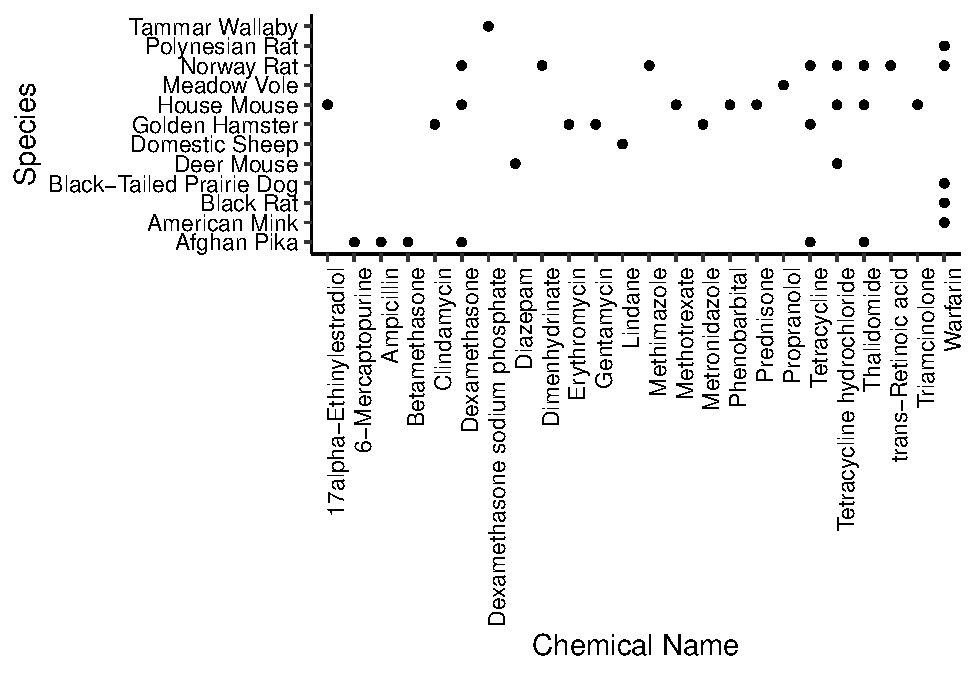
\includegraphics{Reents_ENV872L_Project_files/figure-latex/Exploratory 1-1.pdf}
\caption{Figure 1: Exploratory visualization 1, species tested for each
chemcial}
\end{figure}

\begin{figure}
\centering
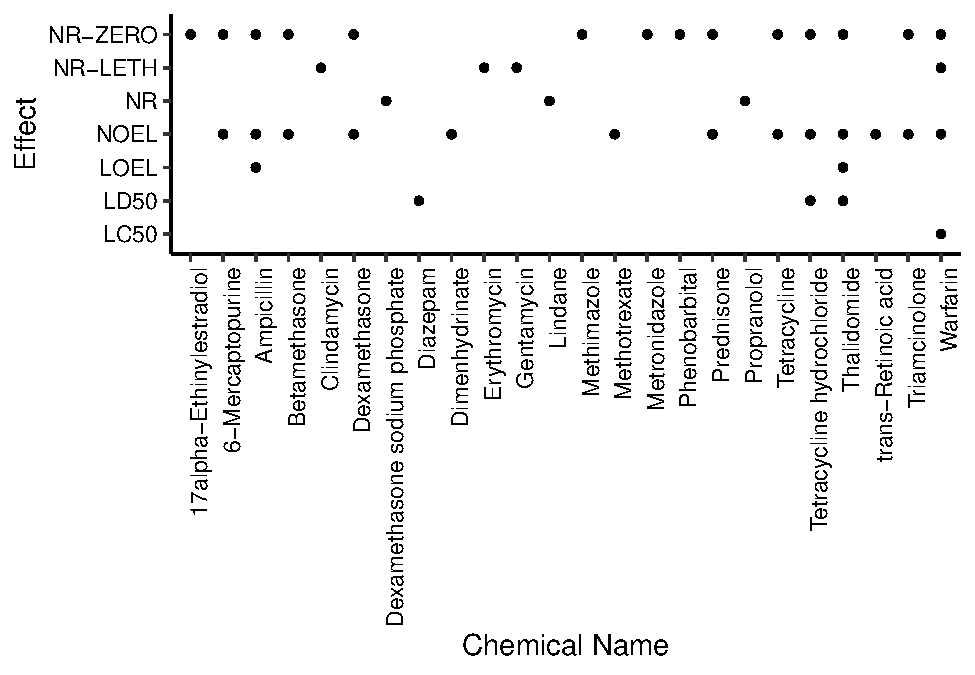
\includegraphics{Reents_ENV872L_Project_files/figure-latex/Exploratory 2-1.pdf}
\caption{Figure 2: Exploratory visualization 2, endpoint effects for
each chemical}
\end{figure}

\begin{figure}
\centering
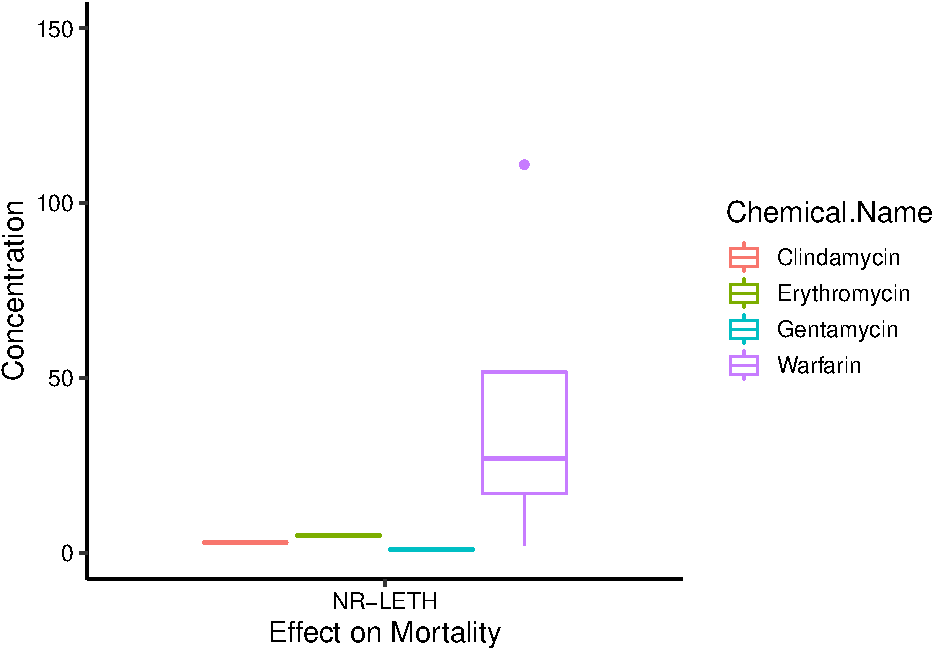
\includegraphics{Reents_ENV872L_Project_files/figure-latex/exploratory 3-1.pdf}
\caption{Figure 3: Exploratory visualization 3, concentration of drugs
assocaited with 100\% mortality}
\end{figure}

The first exploratory graph shows which drugs were tested on which
animals. This helps visualize if each drug was tested on each animal,
which could effect the results of certain statistical tests. For the
second exploratory figure, I wanted to see which drugs resulted in which
endpoints. I was particulary interested to see which drugs resulted in
100\% mortality (NR-LETH). For the third exploratory figure, I
determined the spread of concentration for the drugs that caused 100\%
mortality (NR-LETH). I wanted to determine if certain drugs required
higher concentrations to kill and if certain drugs killed at multiple
concentrations.

\newpage

\section{Analysis}\label{analysis}

\begin{Shaded}
\begin{Highlighting}[]
\KeywordTok{chisq.test}\NormalTok{(}\KeywordTok{table}\NormalTok{(Mammal_dat_RAW}\OperatorTok{$}\NormalTok{Drug.Class, Mammal_dat_RAW}\OperatorTok{$}\NormalTok{Endpoint), }\DataTypeTok{correct =} \OtherTok{FALSE}\NormalTok{)}
\end{Highlighting}
\end{Shaded}

\begin{verbatim}
## Warning in chisq.test(table(Mammal_dat_RAW$Drug.Class,
## Mammal_dat_RAW$Endpoint), : Chi-squared approximation may be incorrect
\end{verbatim}

\begin{verbatim}
## 
##  Pearson's Chi-squared test
## 
## data:  table(Mammal_dat_RAW$Drug.Class, Mammal_dat_RAW$Endpoint)
## X-squared = 48.352, df = 12, p-value = 2.714e-06
\end{verbatim}

\begin{Shaded}
\begin{Highlighting}[]
\KeywordTok{chisq.test}\NormalTok{(}\KeywordTok{table}\NormalTok{(Mammal_dat_RAW}\OperatorTok{$}\NormalTok{Common.Name, Mammal_dat_RAW}\OperatorTok{$}\NormalTok{Endpoint), }\DataTypeTok{correct=}\OtherTok{FALSE}\NormalTok{)}
\end{Highlighting}
\end{Shaded}

\begin{verbatim}
## Warning in chisq.test(table(Mammal_dat_RAW$Common.Name,
## Mammal_dat_RAW$Endpoint), : Chi-squared approximation may be incorrect
\end{verbatim}

\begin{verbatim}
## 
##  Pearson's Chi-squared test
## 
## data:  table(Mammal_dat_RAW$Common.Name, Mammal_dat_RAW$Endpoint)
## X-squared = 228.26, df = 66, p-value < 2.2e-16
\end{verbatim}

\begin{Shaded}
\begin{Highlighting}[]
\NormalTok{mylogit <-}\StringTok{ }\KeywordTok{glm}\NormalTok{(Endpoint }\OperatorTok{~}\StringTok{ }\NormalTok{Conc..Mean..Std., }\DataTypeTok{data =}\NormalTok{ Mammal_dat_RAW, }\DataTypeTok{family =} \StringTok{"binomial"}\NormalTok{)}
\end{Highlighting}
\end{Shaded}

\begin{verbatim}
## Warning: glm.fit: fitted probabilities numerically 0 or 1 occurred
\end{verbatim}

\begin{Shaded}
\begin{Highlighting}[]
\KeywordTok{summary}\NormalTok{(mylogit)}
\end{Highlighting}
\end{Shaded}

\begin{verbatim}
## 
## Call:
## glm(formula = Endpoint ~ Conc..Mean..Std., family = "binomial", 
##     data = Mammal_dat_RAW)
## 
## Deviance Residuals: 
##      Min        1Q    Median        3Q       Max  
## -2.45219   0.00522   0.07686   0.52885   0.61042  
## 
## Coefficients:
##                  Estimate Std. Error z value Pr(>|z|)   
## (Intercept)       1.58576    0.50945   3.113  0.00185 **
## Conc..Mean..Std.  0.01413    0.01126   1.255  0.20956   
## ---
## Signif. codes:  0 '***' 0.001 '**' 0.01 '*' 0.05 '.' 0.1 ' ' 1
## 
## (Dispersion parameter for binomial family taken to be 1)
## 
##     Null deviance: 45.016  on 96  degrees of freedom
## Residual deviance: 35.578  on 95  degrees of freedom
## AIC: 39.578
## 
## Number of Fisher Scoring iterations: 14
\end{verbatim}

It was difficult to run statistical tests on this data because I was
working with mostly categorical data. This is why I chose to run chi
squared tests and a logit glm. While the chi squared test warns that it
may not be accurate due to sample size, I still ran it and cited it as
the findings were seen in the visual aides. That said, it is important
to note that these finidings may nt be statistically significant, which
is probably because many drugs or species had limited studies done on
them. I had to use a binomial glm because the dependent variable was
categorical.

\begin{figure}
\centering
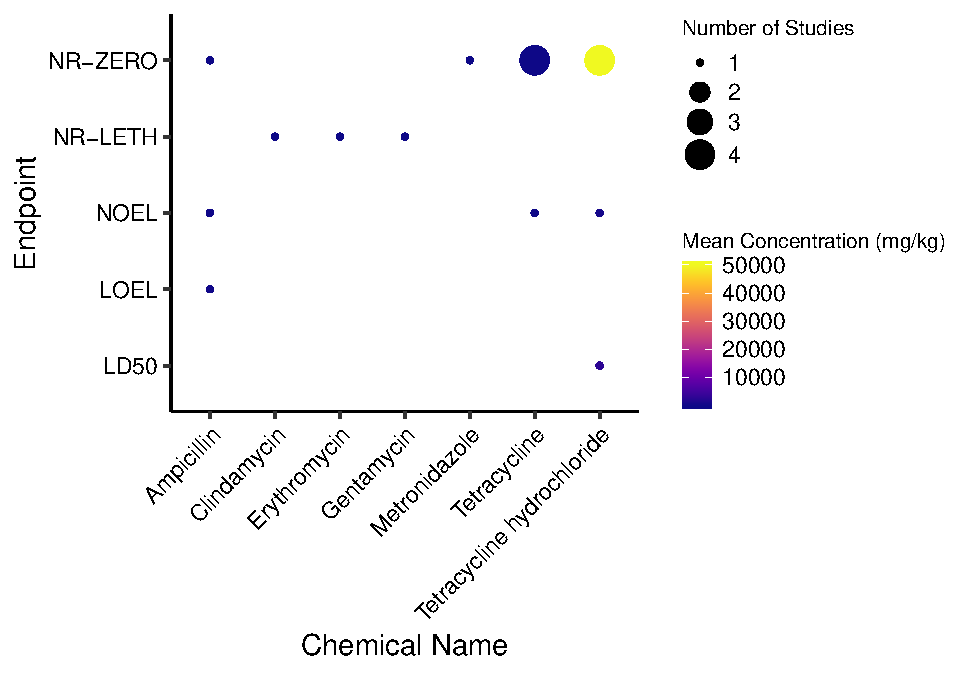
\includegraphics{Reents_ENV872L_Project_files/figure-latex/visualization 1-1.pdf}
\caption{Figure 4: Antibiotics and their endpoints based on
concentration. Larger dots indicate more studies.}
\end{figure}

\begin{verbatim}
## Warning: Ignoring unknown parameters: breaks
\end{verbatim}

\begin{figure}
\centering
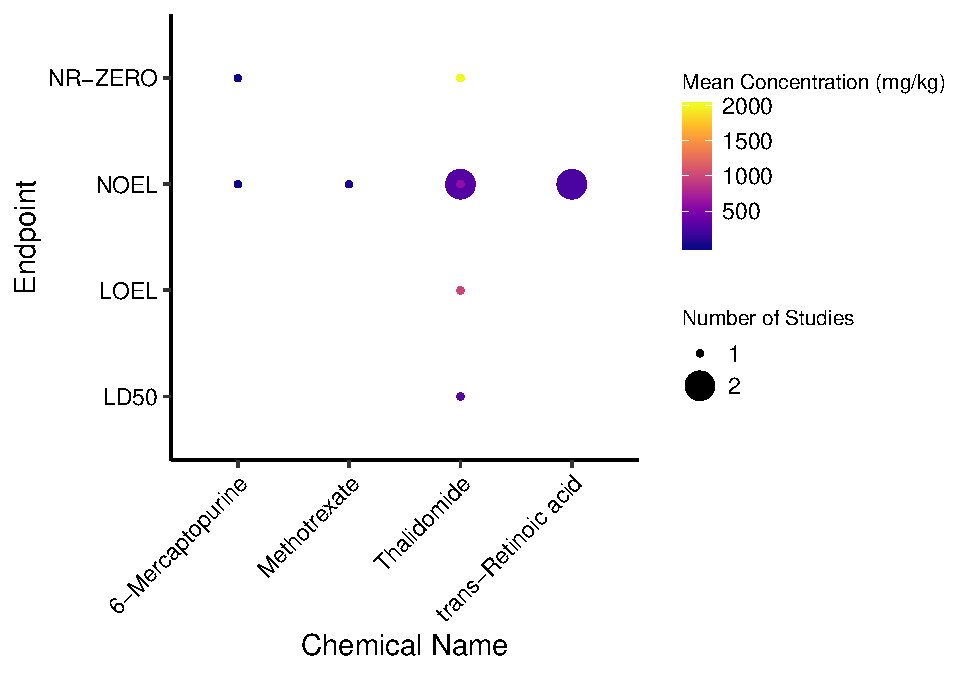
\includegraphics{Reents_ENV872L_Project_files/figure-latex/visualization 2-1.pdf}
\caption{Figure 5: Anti-cancer drugs and their endpoints based on
concentration. Larger dots indicate more studies.}
\end{figure}

\begin{figure}
\centering
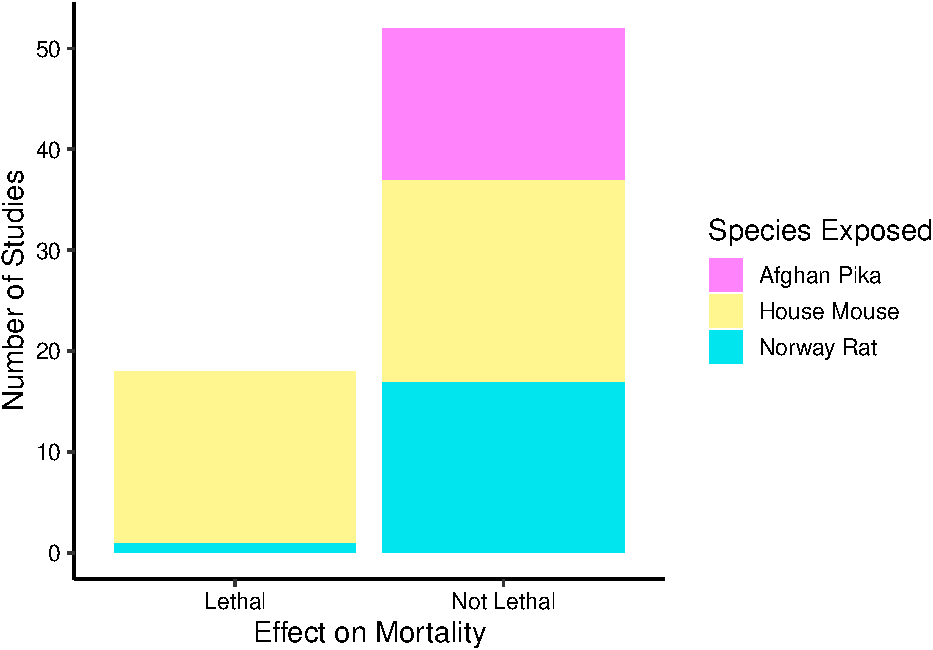
\includegraphics{Reents_ENV872L_Project_files/figure-latex/Visualization3-1.pdf}
\caption{Figure 6: Top three most studied organisms and the number of
studies which proved lethal for that organism. `Lethal' includes LD50
(50\% morality) and NR-LETH (100\% mortality), `Not Lethal' includes
measures with minimal or no effect on the organism.}
\end{figure}

\begin{figure}
\centering
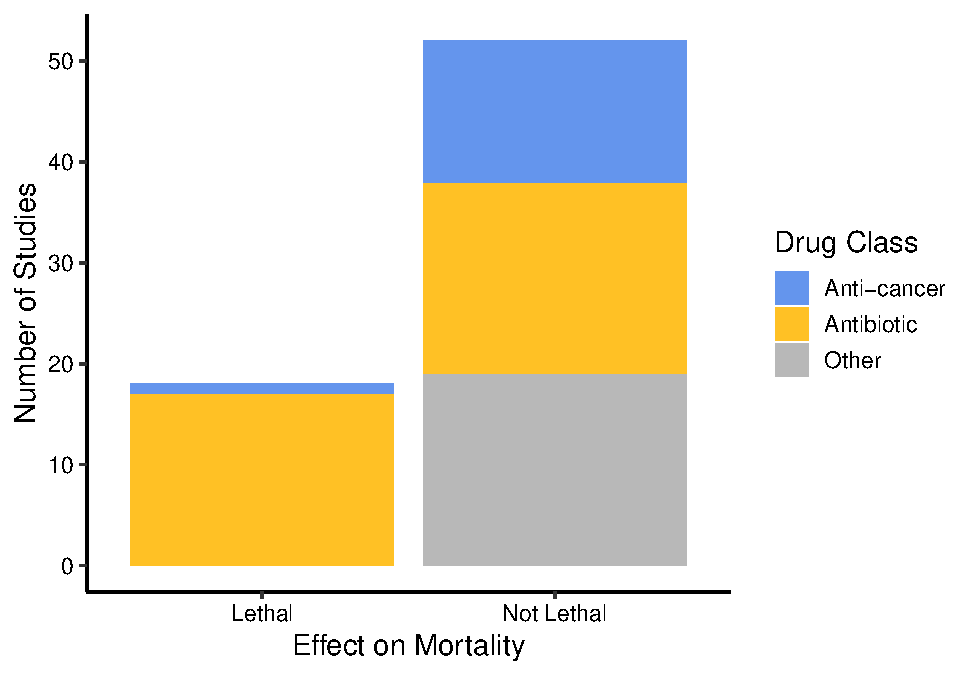
\includegraphics{Reents_ENV872L_Project_files/figure-latex/visualization4-1.pdf}
\caption{Figure 7: Number of studies associated with each drug class and
whether or not they proved lethal. Again, `Lethal' includes LD50 (50\%
morality) and NR-LETH (100\% mortality), `Not Lethal' includes measures
with minimal or no effect on the organism.}
\end{figure}

\begin{figure}
\centering
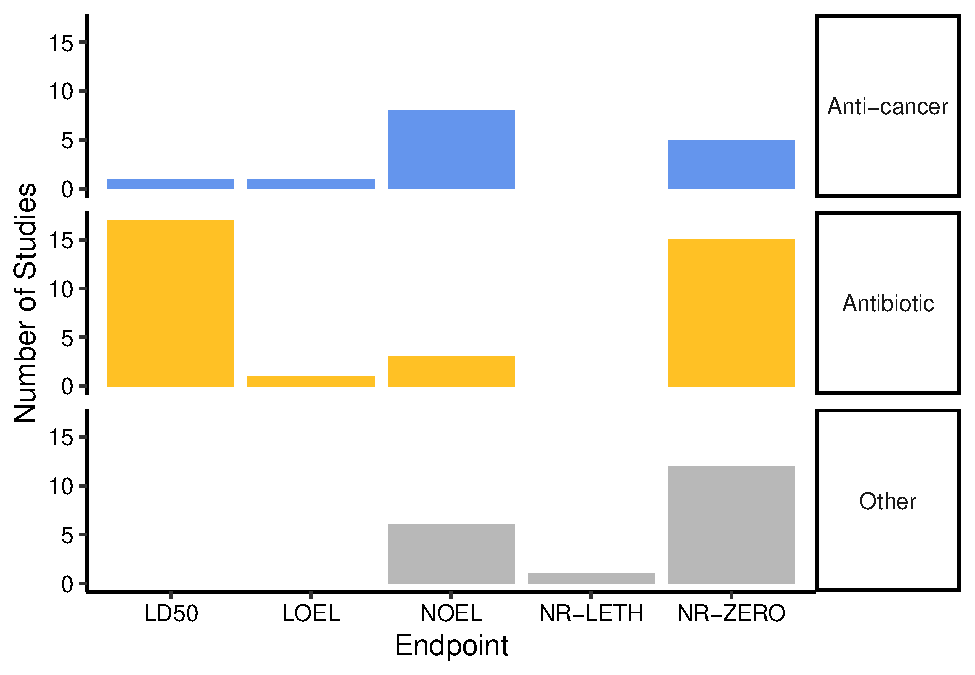
\includegraphics{Reents_ENV872L_Project_files/figure-latex/visualization5-1.pdf}
\caption{Figure 8: Endpoint effects of each drug class dependent on how
many studies came to the same conclusion.}
\end{figure}

Figure 4+5: The goal of visualization one and two is to visualize both
the concentrations of the different drugs associated with the different
endpoints, but also how many studies were done on that drug. Presumably
the bigger the dot the more robust that data point because it is based
off of many studies instead of just one.

Figure 6: The goal here is to briefly visualize the proportion of
studies that were lethal to which of the three most tested organisms. I
excluded animals that were not studied as often, so that the results are
more robust.

Figure 7:The goal of this graph is similar to the previous one, but I
wanted to visualize the proportion of studies found to be lethal or not
for each drug class. While it is not based on proportions, it is still a
good visual to gague how many studies total found each outcome and which
drugs were tested in those studies.

Figure 8: In this figure I wanted to further break down and see each end
point seperately. Mainly because there is an important difference from
50\% mortality to 100\% mortality.

\newpage

\section{Summary and Conclusions}\label{summary-and-conclusions}

Through my statistical tests, I found a few patterns in the data. By
running a chi squared test to determine the relation between drug class
and endpoint, I found that the class of drug is related to the endpoint
(p\textless{}0.05). This means that whether a drug is an antibiotic,
anti-cancer drug, or ``other'' is associated with the morotality of the
test organsims. By looking at (Figure 7), you can see that of the
studies finding lethal effects, most were antibiotics.

Another chi squared test found that the relationship between species
tested and mortality rates was also significantly associated
(p\textless{}0.05). This means that certain species experienced
different effects than others. Of course, this may be just due to the
fact that each drug was not tested on each organism. By looking at
(Figure 6), you can see that of the studies that found lethal effects,
most were tested on the common house mouse.

Through running a logit model, I did find that concentration was not a
significant predictor of endpoint (p\textgreater{}0.05). Applying this
to the issue of water contamination, this may mean that concentrations
will not effect how contamination effects animals. Depending on the drug
this maay be good or bad. This may mean that small doses of chemicals
have the same effect as large doses, so while we don't need to worry
about concentrations getting higher, it is clear that we need to worry
about the concentrations that are already present. Looking at Figure 4
you can see that most drugs were test in low concentrations. It is
interesting to note that the top two most studied drugs had zero
mortality and the ones that proved lethal had less studies associated
with them. Loojing at tetracycline hyrdrochloride I find it interesting
that a lower concentration had the LD50 effect, which indicates 50\%
mortality, while the higher concentration was associated with zero
mortality. By loking at Figure 5 you can see that none of the
anti-cancer drugs caused 100\% mortality, the only lethality was seen in
one study on Thalidomide (LD50- 50\% mortality). Looking at Figure 8 you
can see again that antibitics causes the most lethal outcomes. I was
surprised by these findings, I expected that anti-cancer drugs, like
Methotrexate would have more lethal effects than antibiotics.


\end{document}
